% $Id%

% ++++++++++++++++++++++++++++++++++++++++++++++++++++++++++++++++++++++++++
%\pagebreak
\newpage
\enlargethispage{1cm}
\hypertarget{appendix-menutree}{}
\section{CrypTool Menus}
\label{s:appendix-menutree}

This appendix contains at the following page the complete menu tree of
CrypTool\index{CrypTool} version 1.4.31\footnote{%
  In parallel to CrypTool 1.x (CT1)\index{CrypTool 1.x} the future versions
  CrypTool 2 (CT2)\index{CrypTool 2.0} and JCrypTool (JCT)\index{JCrypTool 1.0}
  are currently developed in the CrypTool project.\\
  - Webseite CT2: \url{http://www.cryptool2.vs.uni-due.de} \\
  - Webseite JCT: \url{http://jcryptool.sourceforge.net} \\
  These future versions are currently (July 2012) beta versions, but they
  are stable enough to be used by end-users already.\\
}. 

\noindent The main menu of CT1 contains service functions in the menus
\begin{itemize}
   \item File
   \item Edit
   \item View
   \item Options
   \item Window
   \item Help
\end{itemize}
and the actual cyrpto functions in the menus
\begin{itemize}
   \item Encrypt/Decrypt
   \item Digital Signature/PKI
   \item Individual Procedures
   \item Analysis.
\end{itemize}

Below \verb#Individual Procedures# you find visualizations of single algorithms
and of protocols. Some procedures are implemented both for a fast performance
(mostly under the main menu \verb#Encrypt/Decrypt#) and for a step-by-step visualization.

Which menu items in CrypTool are active (that means not greyed), depends on
the type of the currently active document window:
The brute-force analysis\index{Attack!brute-force} for DES e.~g. is only
available, if the active window is opened in the hexadecimal view. 
On the other hand the menu item ``Generate Random Numbers\dots''
is always available (even if no document is opened).

%The following four types of documents exist in CrypTool:
%\begin{center}
%\begin{tabular}{rl}
%\bf Code letter & \bf Type of document \\
%T & Text file view\\
%H & Hexadecimal view\\
%P & Diagram/plot view (histogram, autocorrelation)\\
%O & OpenGL graphics view\\
%\end{tabular}
%\end{center}


%\nobreak
\clearpage
\begin{figure}[hb]
\begin{center}
\vspace{-30pt}
%\frame{  %TeX macht einen Rahmen (siehe viewport) drumherum -- gut zum Testen
%\includegraphics[scale=0.25, angle=270, viewport=200 30 2660 1430]
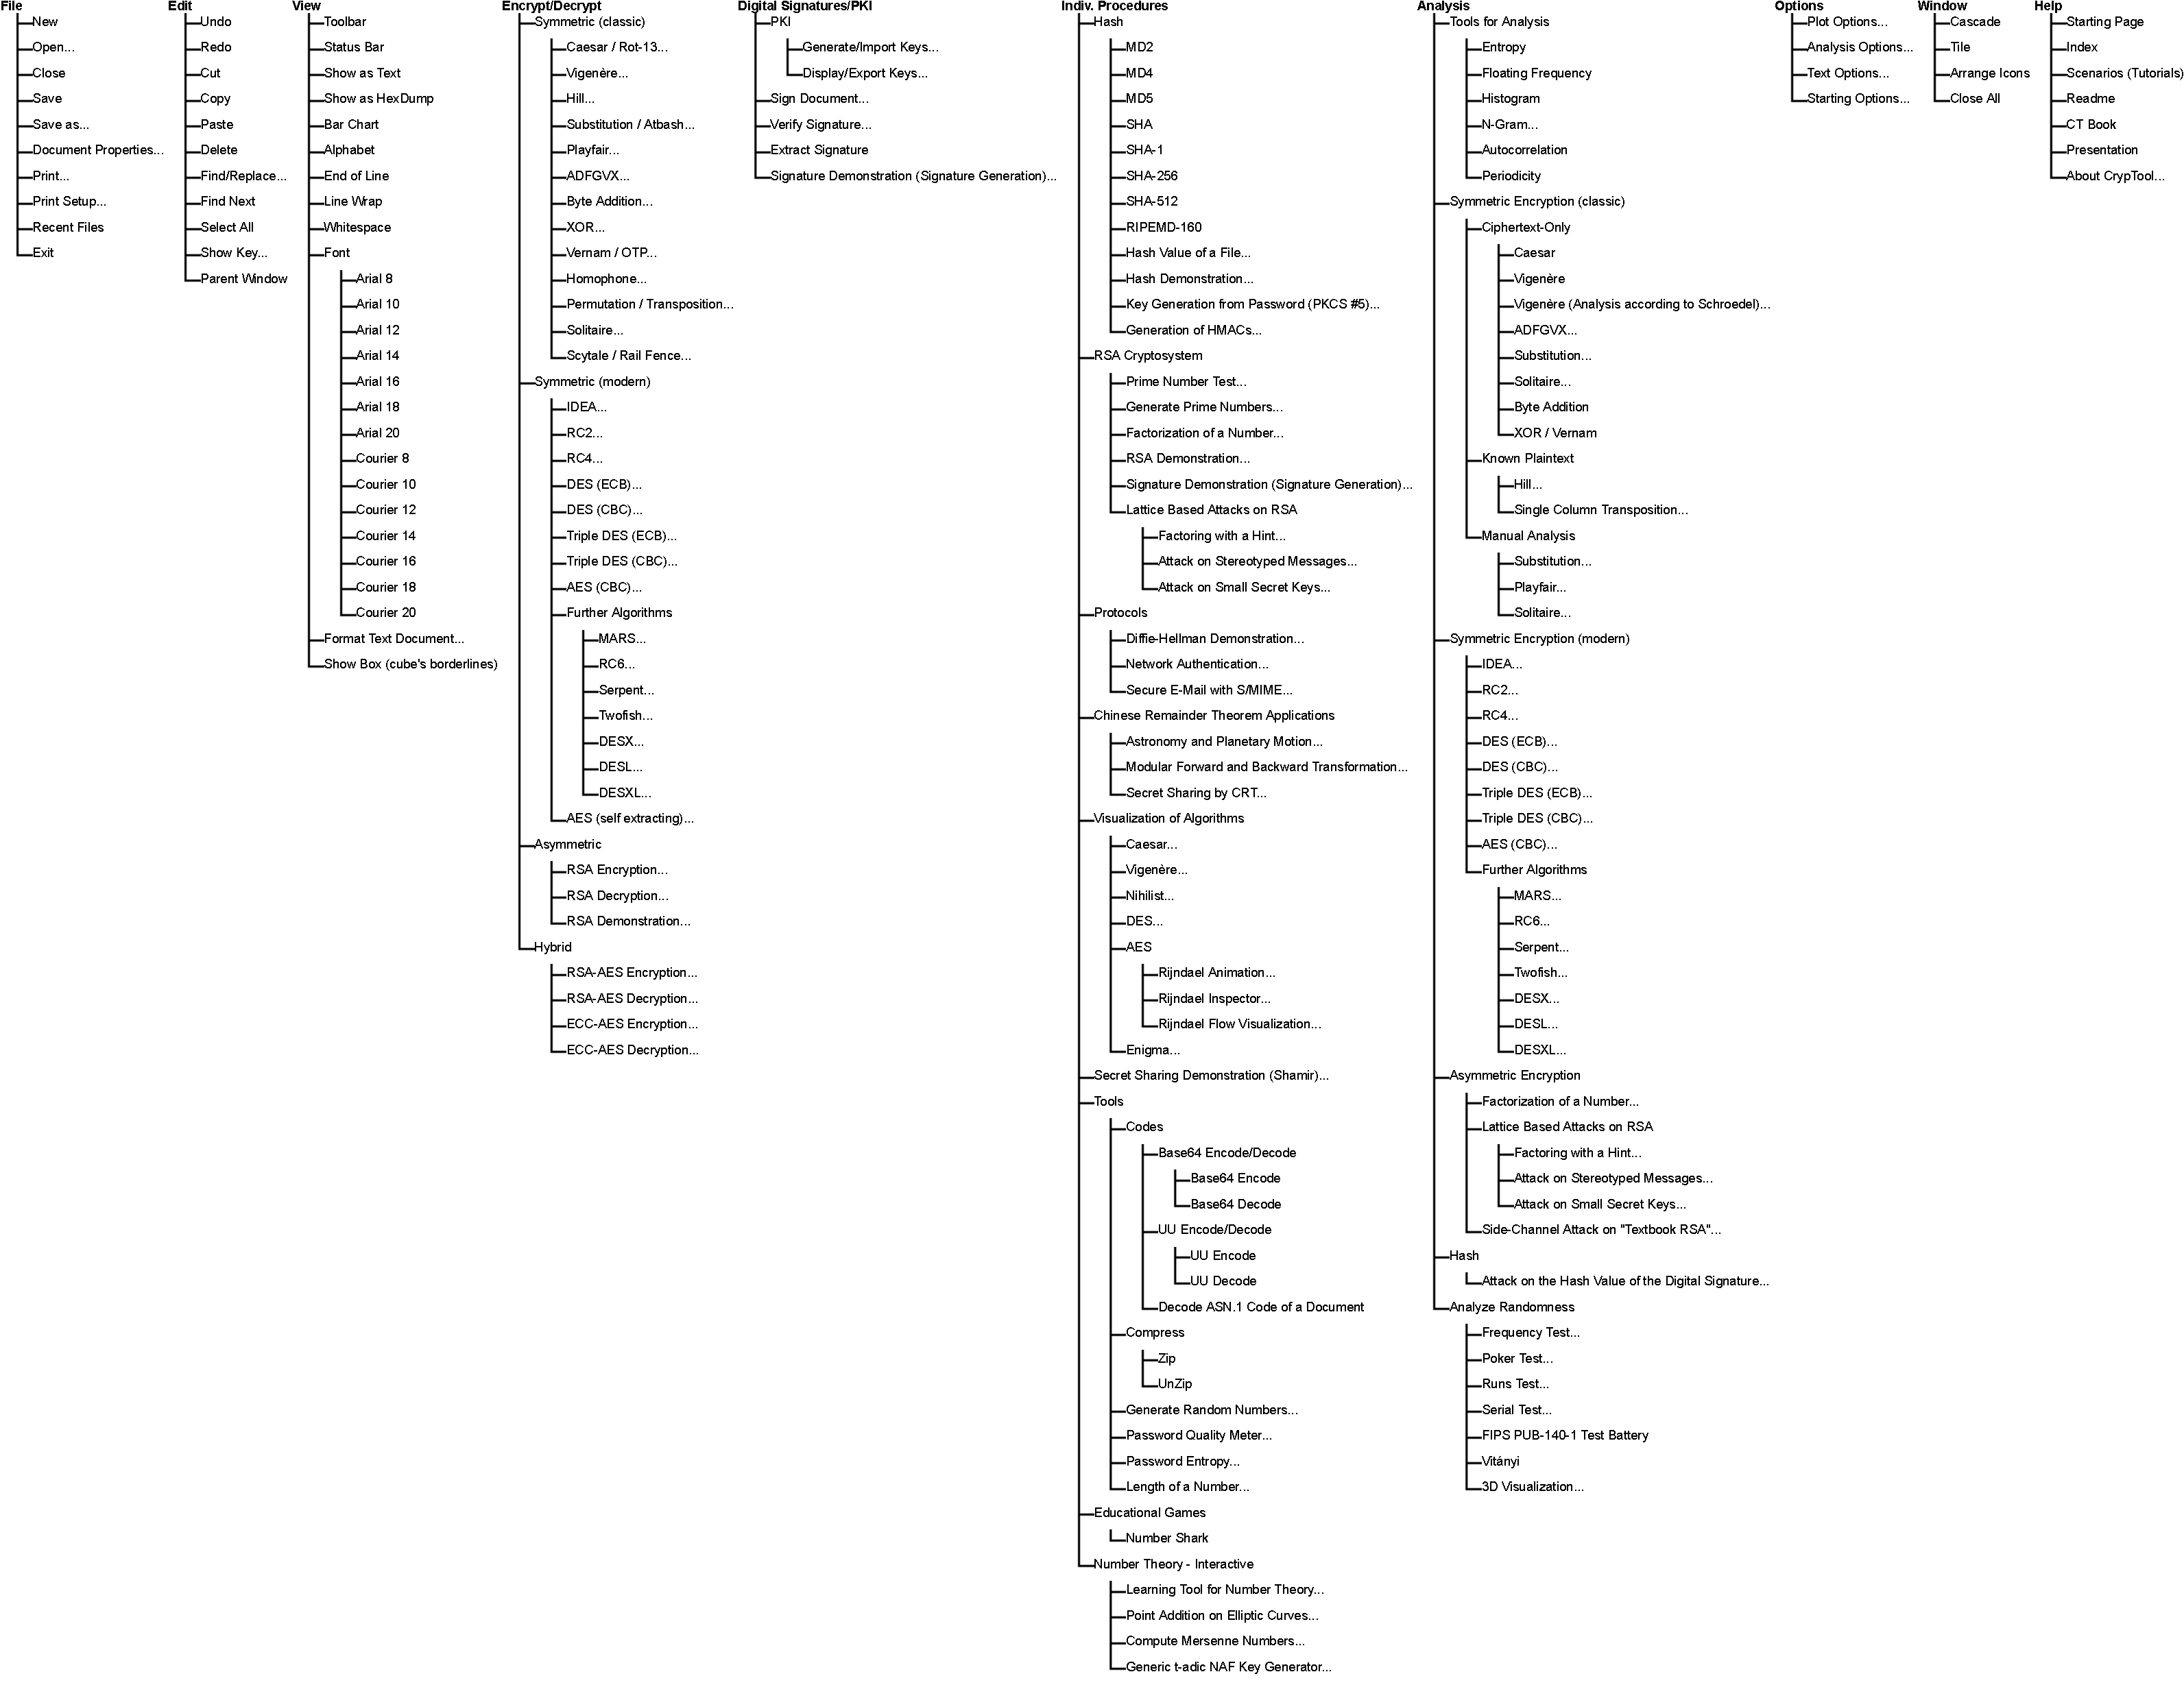
\includegraphics[scale=0.35, angle=270]
                {figures/CT1-menutree-en}
%viewport=rand-links? rand-unten breite hoehe? [bezogen auf querformat]
%}
\caption{Complete overview of the menu tree of CT1 (CrypTool 1.4.31)} 
\label{menuoverview}
\end{center}
\end{figure}
\clearpage


\noindent Text for CT2 xxxxxxxxxx DRAFT

\clearpage
\begin{figure}[hb]
\begin{center}
\vspace{-30pt}
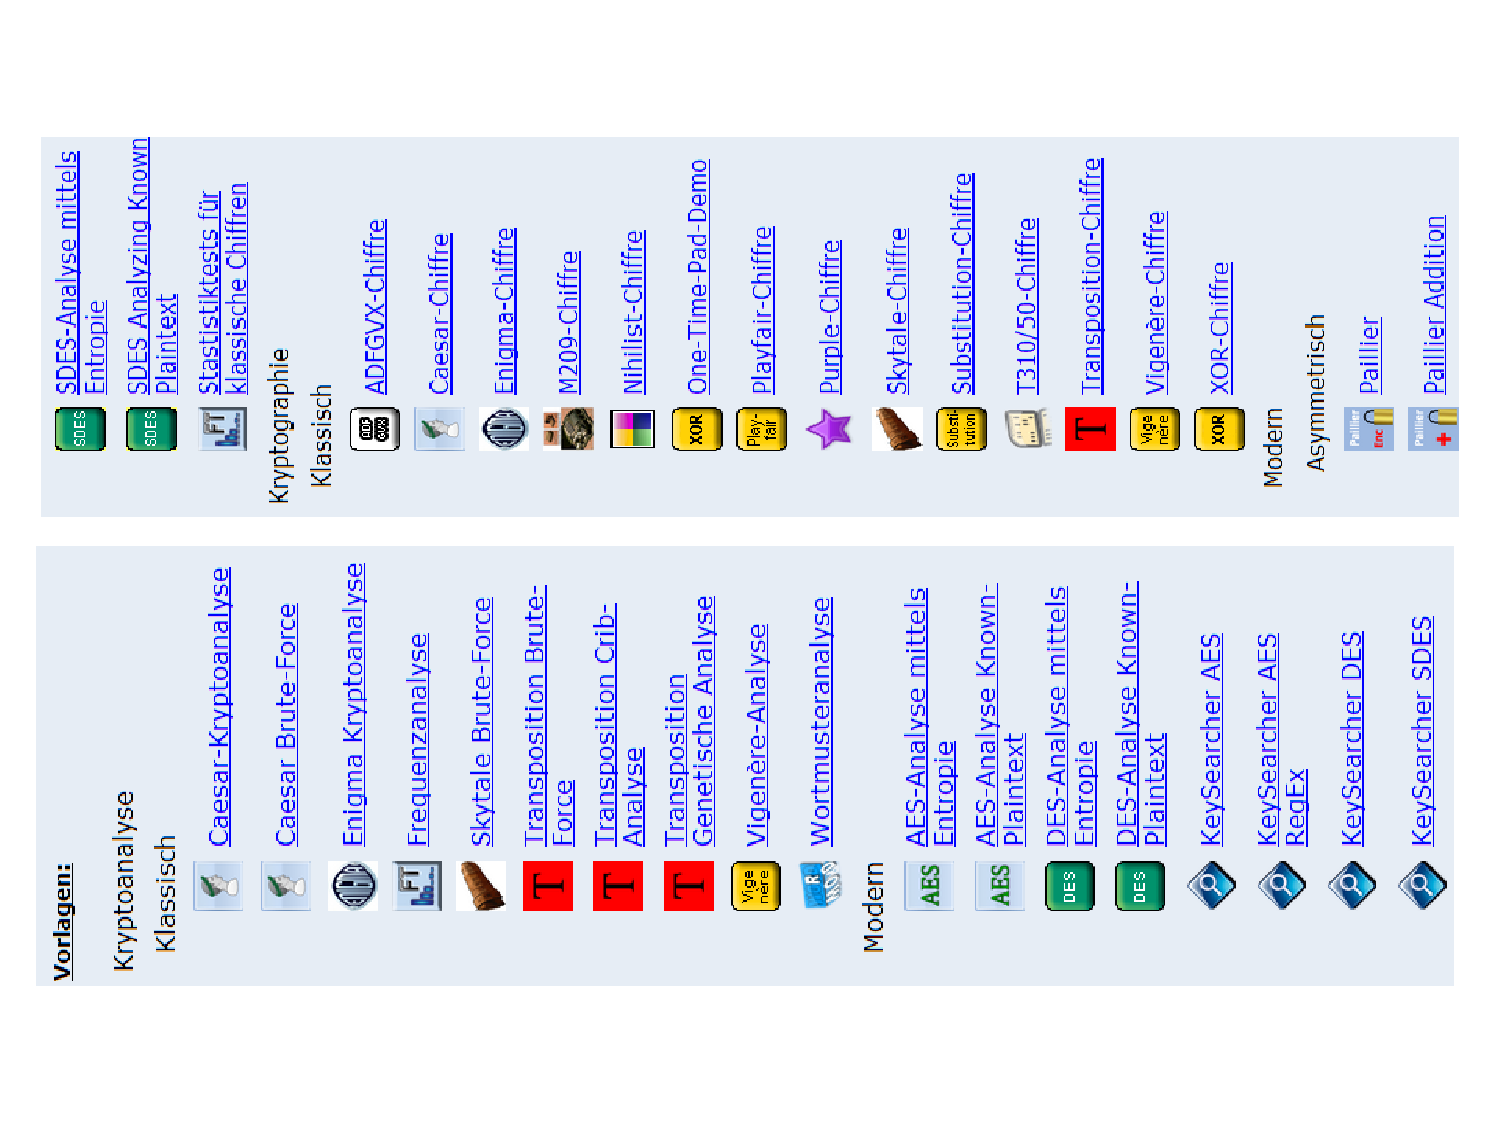
\includegraphics[scale=0.8, angle=270]
                {figures/CT2-templatetree-en}
\caption{Overview of the template tree of CT2 (NB4882.1, July 2012), Part 1} 
\label{menuoverview}
\end{center}
\end{figure}
\clearpage

